\section{Messung}\label{sec:Messung}

Für die in Kapiel \ref{sec:aufbau} gebaute Antenne muss für die Verifikation dessen Funktionsweise ausgemessen werden. Die Resultate werden dabei mit der Simulation aus Kapitel \ref{sec:Simulationsresultate} verglichen. Dieses Kapitel befasst sich mit der Messung der Antenne im Labor.

\subsection{Ideale Messung}

Um eine Antenne vermessen zu können müssen ideale Bedingungen erfüllt werden. Bereits kleine Imperfektionen können zu Störungen führen. Die Bedingungen sind dabei davon abhängig, welche Eigenschaft der Antenne ausgemessen werden soll.
Für ideale Messungen werden reflexionsarme Räume bevorzugt \cite{ranges}. Diese Räume sind so aufgebaut, dass elektromagnetische Wellen an den Wänden und dem Boden absorbiert werden. Da der Abstand von der Empfängerantenne zur Testantenne für Fernfeldmessungen in der Regel mehrere Wellenlängen betragen muss ($R > \frac{2D^2}{\lambda} \rightsquigarrow R \gg D$, wobei $R$ den Abstand der Antennen darstellt und $D$ die lineare Dimension der Antenne, siehe Frauenhofer-Distanz \cite{frauenhofer}), werden je nach Antenne sehr grosse Räume benötigt. Daher werden Antennen mit tiefen Frequenzen in der Natur, zum Beispiel in den Bergen, ausgemessen.

\subsection{Messaufbau}

Um die Antenne auszumessen wird der \textit{Network Analyser E5071B} von \textit{Agilent Technoligies} verwendet. Die Antenne wird dabei über einen Adapter am Port 1 des Gerätes angeschlossen.

\begin{figure}[h!]
	\centering
	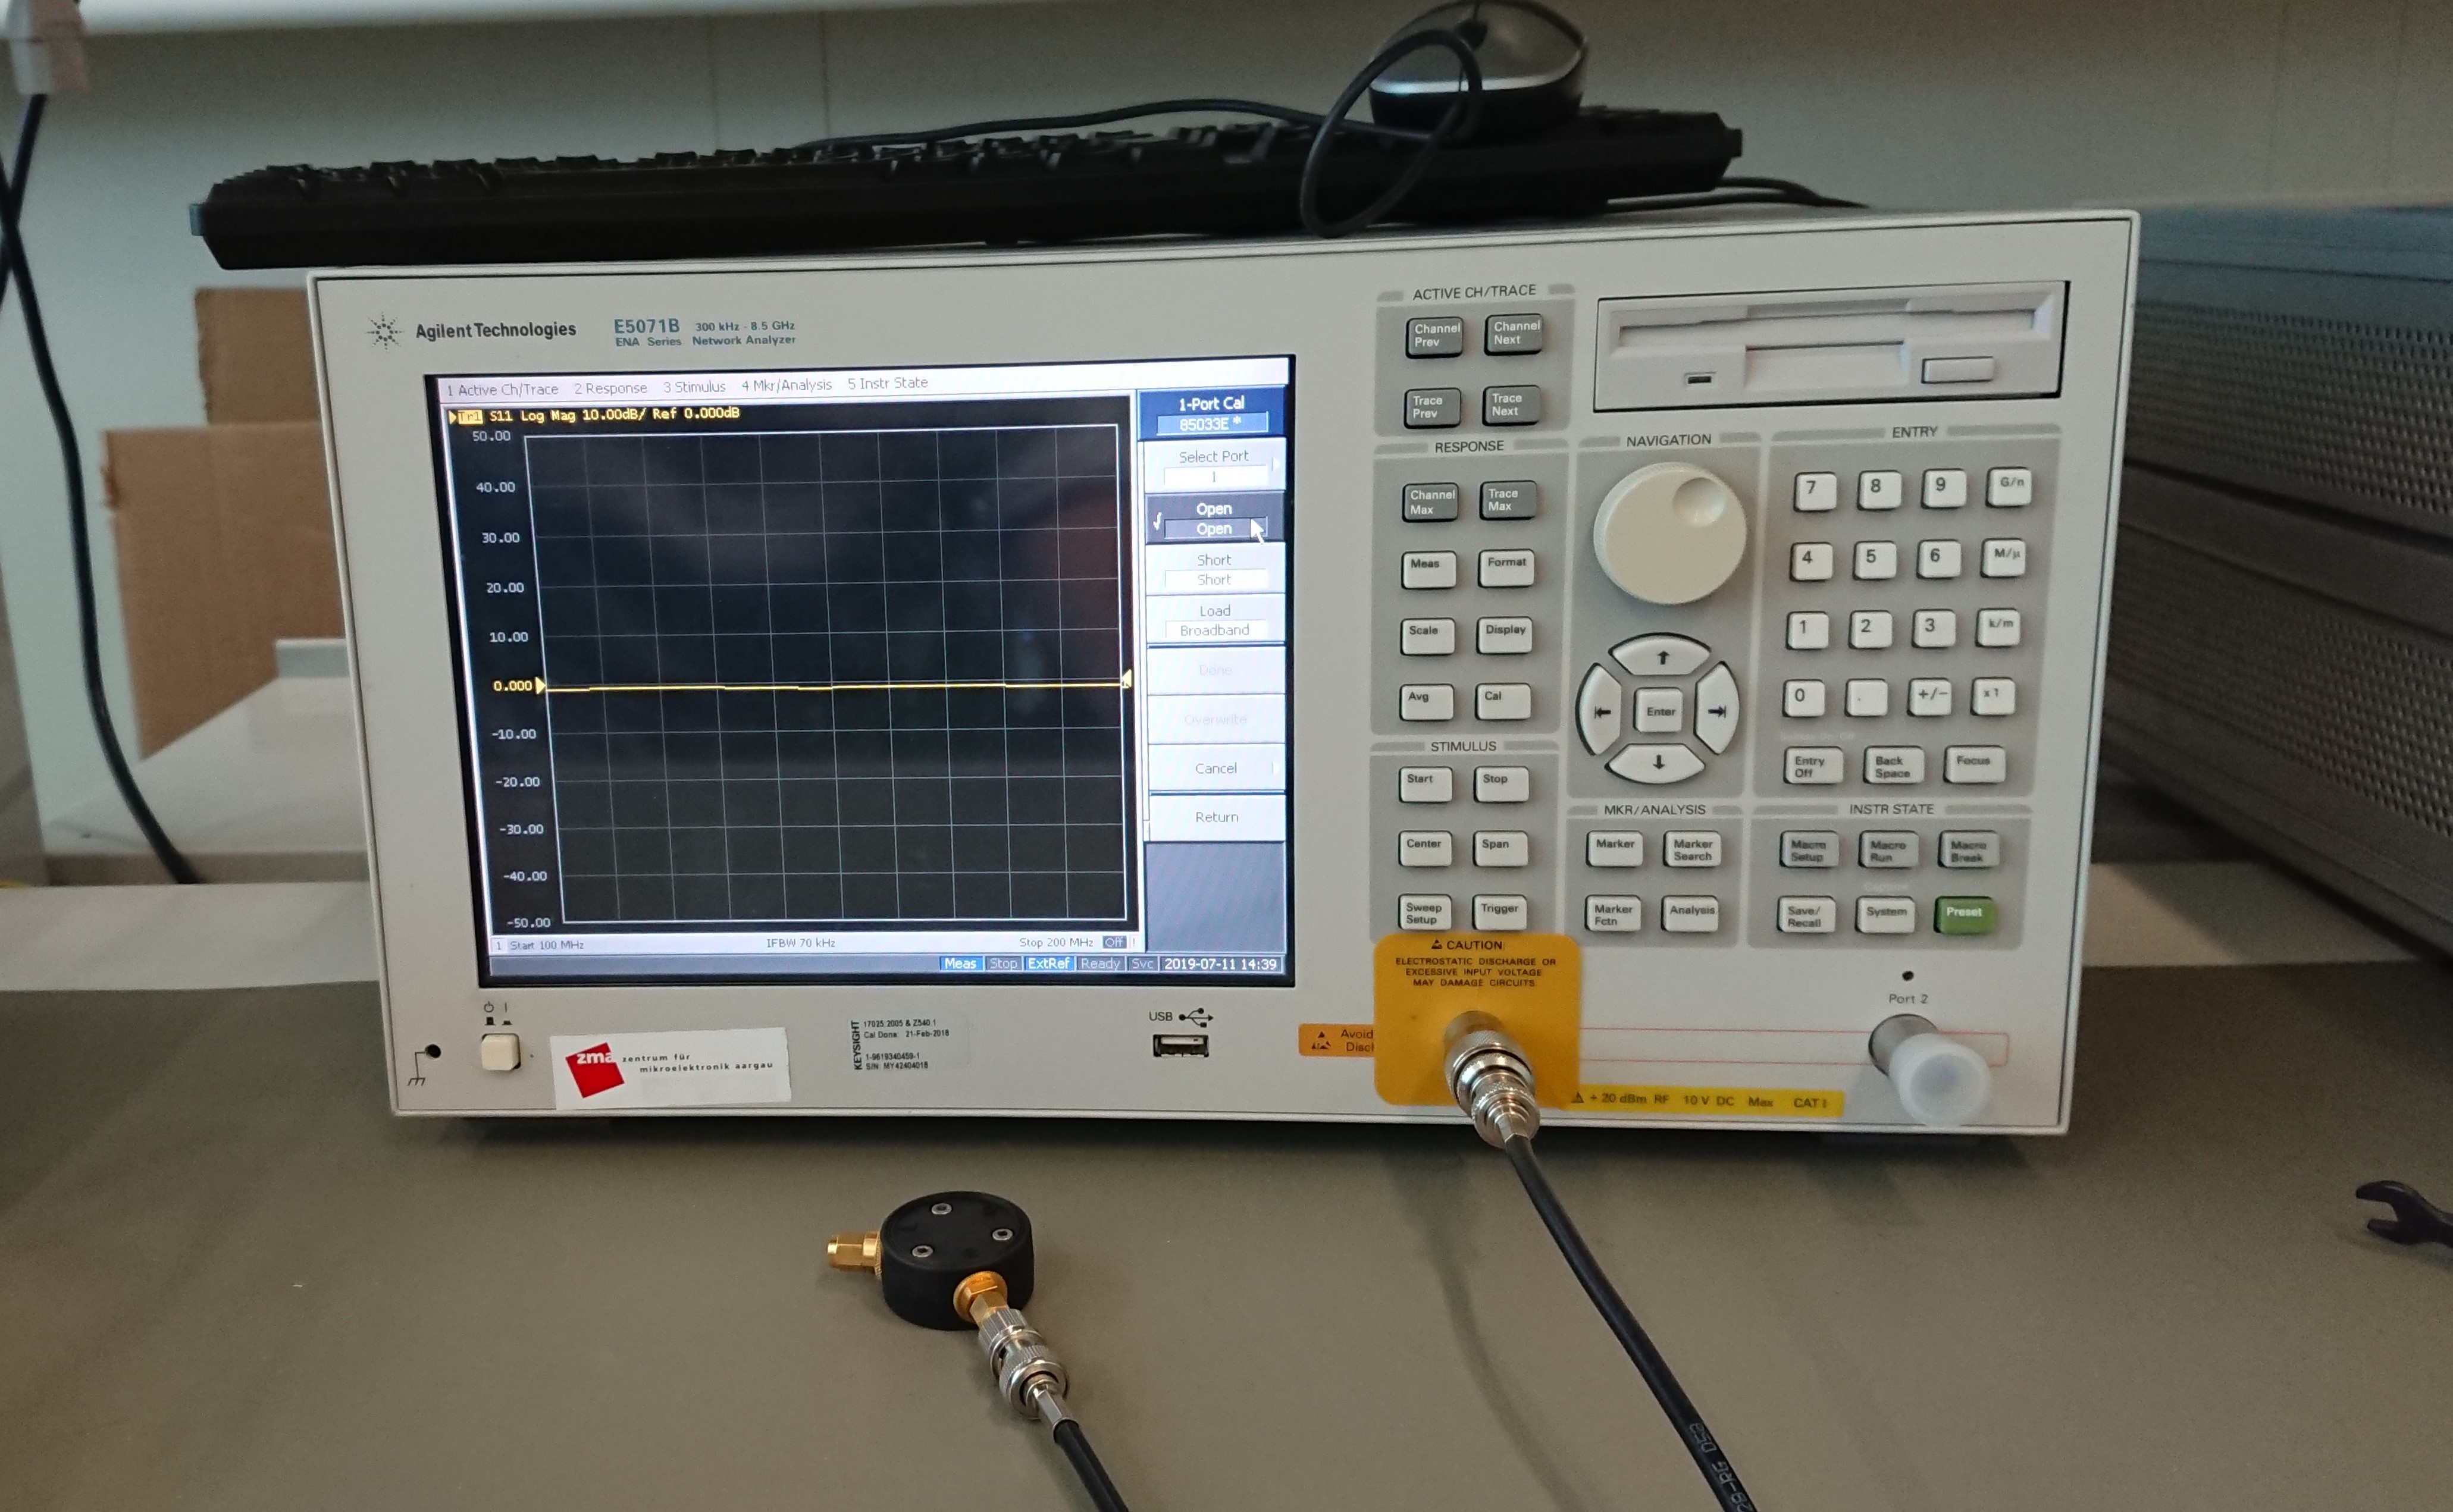
\includegraphics[width=\textwidth/6*5]{Labor2.jpg}
	\caption{Aufbau der Messung mit der Antenne. Im Bild wurde mit dem Element des \textit{Calibration Kits} der Network Analyser kalibriert.}
	\label{fig:Messung_Labor}
\end{figure}

Der Messaufbau ist in Abbildung \ref{fig:Messung_Labor} abgebildet. Hierbei ist jedoch das Element des \textit{Calibration Kits} angeschlossen, welches durch die Antenne ausgetauscht wird.

\subsection{Kalibration des Network Analysers}

Damit die Messungen so genau wie möglich werden muss das Messgerät zuerst kalibriert werden. Da das Koaxkabel der Antenne direkt am Dipol der Yagi-Antenne angelötet ist, muss für die Kalibration ein Kabel bereitgestellt werden. Dieses muss aus dem selben Kabel-Typ wie das der Antenne bestehen und eine identische Länge aufweisen (\SI{2.06}{m}, leicht länger als eine Wellenlänge). Anschliessend wird das \textit{Calibration Kit 85033D} von \textit{Hewlett Packard} verwendet um die Kalibration durchzuführen. Die Kalibration wird manuell mit dem Network Analyser gestarted. Anschliessend wird das eine Ende des \SI{2.06}{m} Koaxkabel über einen passenden Adapter am Port 1 des Network Analysers angeschlossen, während am anderen Ende eines der drei Abschlüsse des \textit{Calibration Kits} entsprechend dem Kalibrationsvorgang angeschlossen. Dabei stehen drei Abschlüsse zur verfügung:

\begin{itemize}
\item Kurzschluss (S, Short definition)
\item Offener Abschluss (O, Open definition)
\item Abschlusswiderstand (L, Load definition)
\end{itemize}

Diese Abschlüsse sind in Abbildung \ref{fig:Messung_Abschluss} aufgeführt. Die Kalibration muss dabei über einen angemessen Bereich durchgeführt werden, welcher für die Yagi-Antenne auf \SI{100}{MHz} bis \SI{200}{MHz} eingestellt wurde. Nach dieser Kalibration kann die Antenne ausgemessen werden. Der kalibrierte Network Analyser ist unter dem Messaufbau in Abbildung \ref{fig:Messung_Labor} abgebildet, was anhand der konstanten Dämpfung identifizierbar ist.

\begin{figure}[h!]
	\centering
	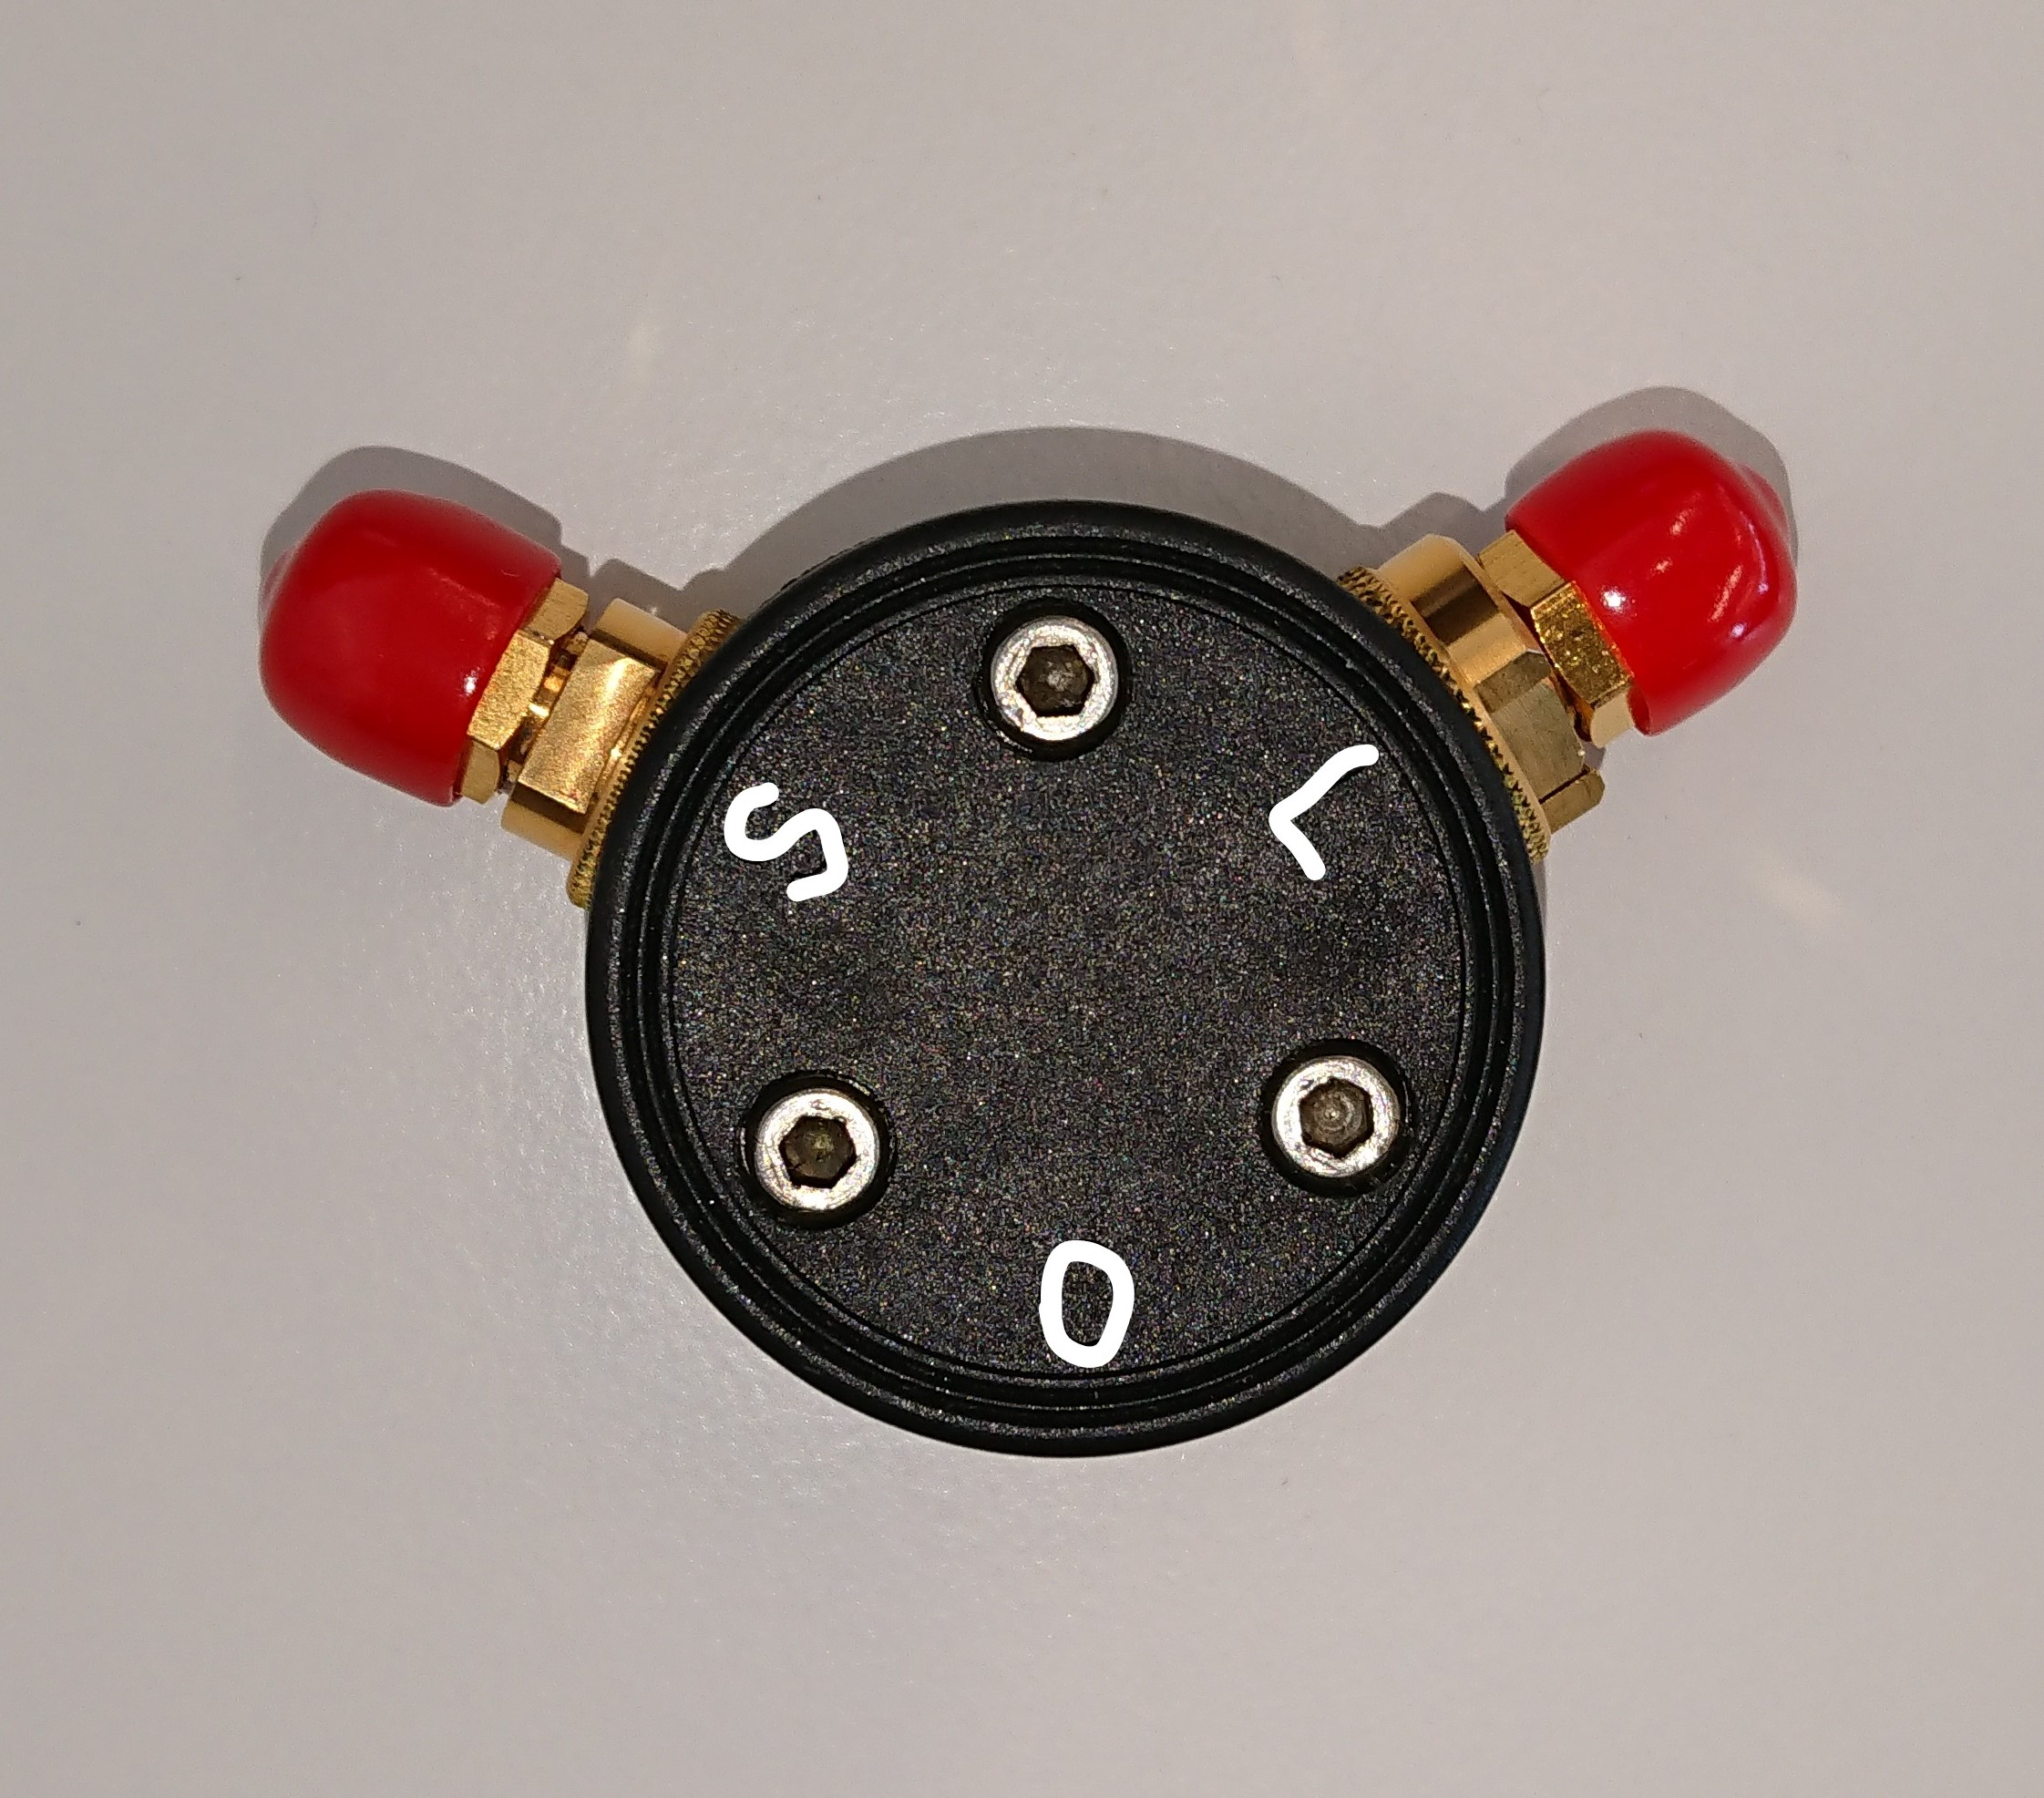
\includegraphics[width=\textwidth/4]{Abschluss.jpg}
	\caption{Element des \textit{Calibration Kits} mit allen drei Abschlüssen. Der offene Abschluss wurde dabei entfert und dessen Messung kann ohne Abschluss durchgeführt werden.}
	\label{fig:Messung_Abschluss}
\end{figure}


\subsection{Messung der Antenne im Labor}

Da kein reflexionsarmer Raum zu Verfügung steht muss die Antenne entweder im Freien oder im Labor des ISE ausgemessen werden. Dabei wurde das Labor ausgewählt um den Transport der Messgeräte zu vermeiden. Das Labor besteht jedoch aus sehr vielen Störquellen, weshalb die Ausmessung der Antenne nur als verifikation der Funktionsweise angesehen werden soll.\\
Bei der Messung ist jedoch relativ schnell klar geworden, dass kleine Änderungen der Ausrichtung der Antenne schon grosse Schwankungen aufzeigen. Bei der Messung ist daher wichtig, die Antenne stabil zu halten oder zu befestigen.

\newpage

\begin{figure}[!ht]
\centering
\begin{tikzpicture}
%\selectcolormodel{gray}
\begin{axis}[xmin=100e6,   xmax=200e6,
			 	   ymin=-43,   ymax=5,
			 	   title=Measurement S11 Parameter Yagi-Antenna,
			 	   xlabel=Frequency (Hz),
				   ylabel=Gain (dB),
				   grid=both,
				   width=15cm,height=12cm,
				   scaled ticks=engineering,
				   legend cell align=left,
			 	   legend pos=north east,
				   ]
\addplot[red] table [mark=none, x=f, y=dB, col sep=comma] {csv/S11.csv};
\addlegendentry{S11 Yagi-Antenna}
\end{axis},
\end{tikzpicture}
\caption{Messung der Yagi-Uda-Antenne im Labor mit dem Network Analyser.}
\label{fig:Messung_S11}
\end{figure}

Abbildung \ref{fig:Messung_S11} zeigt die gemessenen S1,1 Parameter der gebauten Antenne im Labor. Die Auflösung der exportierten Datenpunkte ist nicht ganz optimal, da diese in \SI{1}{MHz}-Schritten aufgezeichent wurden, aber es kann eine Grenzfrequenz von \SI{133}{MHz} abgelesen werden. Die Frequenz ist damit identisch zur Frequenz in Kapitel \ref{sec:Simulationsresultate}. Durch die schlechten Messverhältnisse sind Abweichungen zu erwartet gewesen, trotzdem liegt die Frequenz ziemlich genau im selben Bereich. Es muss jedoch auch vermerkt sein, dass wie bereits erwähnt, die Frequenz stark um mehrere Megahertz schwankt (auch bei stabilen Verhältnissen).\\

Weitere Messungen der Antenne wurden nicht durchgeführt, da die Schwankungen während der Messung der S1,1 Parameter zu gross sind, um genaue Schlüsse aus den Resultaten zu ziehen. Zudem ist die Antenne bereits schon etwas deformiert, was nur weitere Ungenauigkeiten liefert.
